\chapter{Forecasting} \label{Chap5}

\section{Forecasting Methodology and Evaluation Metrics}

Forecasting differs from gap-filling in a way that shapes every methodological choice in this
chapter (Chapter~\ref{Chap2}): a forecaster has no access to future context, and predicts forward
recursively from real or previously-predicted history alone. This dissertation evaluates
forecasting exclusively via 365-day recursive rollout from real anchor points -- feeding each
model's own prior-step prediction back in as input for the next step -- rather than one-shot,
fixed-horizon point forecasting, since recursive rollout is the setting a genuine forward-looking
scenario tool (Chapter~\ref{Chap6}) actually requires.

\subsection{Baseline}

Two baselines anchor every result in this chapter: a day-of-year seasonal mean (the historical mean
FCH4 for each calendar day, $\pm$7-day window), and SARIMAX, a classical statistical
time-series model fitted with exogenous meteorological and livestock regressors. seasonal mean is the
baseline against which the primary metric, MASE, is scored throughout this dissertation (D-80,
superseding an earlier chain-persistence convention on the grounds that holding one anchor-day
value flat across a full year is not a baseline a practitioner would ever actually use, regardless
of its own error magnitude); SARIMAX additionally serves as a competitive statistical model in its
own right within the results below.

\subsection{Model Roster}

The tree-ensemble models introduced in Chapter~\ref{Chap4} (Random Forest, XGBoost, LightGBM) and
the tabular foundation models TabPFN and TabICLv2 are reused here in a sequential, recursive-rollout
configuration rather than the tabular gap-filling configuration of Chapter~\ref{Chap4} -- the same
underlying model families, but exercised in the fundamentally different forecasting setting
described above. Two further architectures are introduced specifically for this chapter: the
Temporal Fusion Transformer (TFT), an attention-based sequence model; DLinear, an embarrassingly
simple linear decomposition forecaster motivated by Zeng et al.'s finding that such models can match
or beat far more complex Transformer architectures on standard long-horizon benchmarks
(Section~\ref{sec:tabular-modelling}); and a standard LSTM. An unweighted mean ensemble of Random
Forest, XGBoost, LightGBM, and SARIMAX is also evaluated as a simple, low-effort combination
strategy alongside the individual models.

\subsection{Evaluation Metrics}

MASE (Mean Absolute Scaled Error), scored against the day-of-year seasonal mean baseline above, is
this dissertation's primary forecasting metric throughout, alongside RMSE, WAPE, and Pearson
correlation. $R^2$ is deliberately not reported anywhere in this chapter's forecasting results: on
this spike-dominated, non-stationary target, a handful of extreme-error days can swing $R^2$ by a
large margin without reflecting any real change in forecast skill, making it an unreliable and
non-representative metric for this specific task -- a problem MASE, scored against a like-for-like
seasonal baseline, does not share. (Gap-filling, evaluated on a fundamentally different,
within-distribution interpolation task, does not share this problem and continues to report $R^2$
throughout Chapter~\ref{Chap4}.) One
scoring-convention caveat is stated here, before Section 5.3's results, rather than after: every
result in this chapter is scored against the real observed FCH4 target ($y_{\text{observed}}$), not
the gap-filled series produced in Chapter~\ref{Chap4} ($y_{\text{gapfilled}}$) that seeds each
rollout's autoregressive history. Scoring against $y_{\text{gapfilled}}$ instead reverses the model
ranking reported below (Section 5.3.3), because tree, SARIMAX, and ensemble models are trained by
directly regressing onto that same gap-filled series and so track it circularly well, while TabPFN
and TabICLv2 are evaluated zero-shot against $y_{\text{observed}}$ only and receive no equivalent
boost. $y_{\text{observed}}$ is the metric this dissertation treats as authoritative throughout,
specifically because it is not inflated by this circularity.

\section{Training and Cross-Validation Methodology}

Every rollout result in this chapter uses a 5-anchor sweep -- five distinct real calendar
start-points, each rolled forward 365 days -- rather than a single anchor, since single-anchor
rankings proved unreliable in preliminary checks and do not appear as cited results anywhere in
this chapter. Results are reported pooled across all three towers unless stated otherwise. An
enriched feature set -- species-disaggregated livestock density (cattle/sheep/lamb rather than a
single combined stocking-density figure), a Tower-2 land-use flag, catchment flow, fertiliser-
application recency, and liveweight density -- was constructed uniformly across the full model
roster. Tree, SARIMAX, and ensemble models showed no measurable gain from this enrichment in
preliminary evaluation and were not pursued further given the additional compute cost, so their
results in Section 5.3 use the unenriched base feature set (\texttt{BASE}); foundation and
attention-based models (TabPFN, TabICLv2, TFT, LSTM, DLinear) were evaluated against several
enriched configurations in full, and Table 5.1 reports each model's own best-found configuration
rather than a uniform one across the roster.

\section{Model Results}

\subsection{Full Observed-Target Model Comparison}

\begin{table}[h]
\centering
\footnotesize
\resizebox{\textwidth}{!}{%
\begin{tabular}{@{}l p{7.4cm} c c c c@{}}
\toprule
Model & Hyperparameters / configuration & MASE (seasonal mean) & MAE & WAPE & Correlation \\
\midrule
\textbf{TabPFN} & Blend: p95+25\% spike correction, 1,095d \& 1,460d context windows & \textbf{0.6908} & \textbf{29.82} & \textbf{0.797} & \textbf{0.491} \\
TabICLv2 & 1,460-day context window, tower-robust target scaling & 0.7191 & 30.86 & 0.825 & 0.443 \\
% Ensemble (MASE-weighted) & Inverse-MASE-weighted mean of the RF/XGBoost/LightGBM/SARIMAX rows below & 0.8019 & 34.06 & 0.991 & 0.379 \\
Ensemble & Equal-weighted mean of the RF/XGBoost/LightGBM/SARIMAX rows below & 0.8020 & 34.06 & 0.991 & 0.379 \\
XGBoost & \texttt{max\_depth}=2, \texttt{lr}=0.02, \texttt{n\_estimators}=400, \texttt{min\_child\_weight}=10; full 52-feature enriched set & 0.8038 & 34.02 & 0.988 & 0.364 \\
TFT & \texttt{d\_model}=32, 4 attention heads, \texttt{dropout}=0.1, 28-day lookback; full 52-feature enriched set & 0.8120 & 35.13 & 1.009 & 0.236 \\
LightGBM & \texttt{num\_leaves}=7, \texttt{min\_child\_samples}=10, \texttt{lr}=0.02, \texttt{n\_estimators}=400; driver/livestock-density features only & 0.8166 & 34.81 & 1.014 & 0.371 \\
Random Forest & \texttt{n\_estimators}=500, \texttt{min\_samples\_leaf}=10, \texttt{max\_features}=0.5; driver/livestock-density features only & 0.8411 & 35.17 & 1.045 & 0.380 \\
SARIMAX & AIC-selected order ($p\in\{1,2\}$, $d=1$, $q\in\{0,1\}$ per tower/anchor); driver/livestock-density features only & 0.8741 & 36.11 & 1.082 & 0.348 \\
LSTM & Hidden size 64, 28-day lookback; + species-disaggregated livestock density & 0.9521 & 40.22 & 1.154 & 0.275 \\
DLinear & Trend/seasonal decomposition, kernel=25, 28-day lookback; + bodyweight density & 1.1872 & 45.74 & 1.519 & 0.277 \\
\midrule
\textit{Seasonal Mean (baseline)} & \textit{Day-of-year mean, $\pm$7-day circular window, computed from real pre-anchor history only} & \textit{1.000} & 43.79 & 1.170 & $-0.004$ \\
\bottomrule
\end{tabular}%
}
\caption{Recursive-rollout forecasting results, all-tower pooled, each model's best-selected
configuration. $R^2$ is not reported for forecasting anywhere in this chapter (Section 5.1.3).
\textsuperscript{\dag}WAPE/Correlation for these two B18-refined rows were not part of the B18
refinement pass's own published metrics (Section 5.3.1, below); this dissertation computed them
directly from the underlying saved prediction chains, using the same nine-tower-anchor-block
evaluation set as every other B18 figure, and verified the computation bit-for-bit against the B18
pass's own published MAE and RMSE for both rows before reporting them here. The Seasonal Mean row
is that same climatology baseline's own performance, evaluated on the identical nine-tower-anchor-block
set (n=2,127) as the TabPFN and TabICLv2 rows above; its MASE is 1.000 by definition (a model matching
the baseline exactly). Chain-persistence (the anchor day's real value held flat across the full
365-day rollout) is not used as a MASE reference anywhere in this dissertation (Section 5.1.3).}
\end{table}

TabPFN leads this eleven-model comparison outright, in its standing headline configuration: an
equal-weight blend of three TabPFN variants built on the same \texttt{BASE+ALL} enriched feature set
(52 columns, including species-disaggregated livestock density) used throughout this chapter -- the
model's own p95-quantile spike-excess correction, and two further TabPFN fits trained on shorter,
more recent history windows (1,095 and 1,460 days). Unlike the earlier, un-refined comparison (where
the lowest-MASE model did not also lead on every other metric), the refined TabPFN row is the best
entry in the table on all four columns shown -- MAE, WAPE, and correlation, not only MASE. TabICLv2,
refined the same way (a 1,460-day, tower-robust-scaled variant), moves up to a clear second place,
ahead of every tree, ensemble, and statistical model. Both supersede this dissertation's earlier,
un-refined full-roster entries for these two architectures (TabPFN 0.7149, TabICLv2 0.7385) and beat
the day-of-year seasonal-mean baseline by a wide margin. Among the remaining, un-refined entries,
XGBoost has the lowest MAE (34.02) by a narrow margin over the two ensembles (34.06), and Random
Forest the highest correlation (0.380) -- neither changes the standing result, since MASE remains
the metric this dissertation ranks models by throughout (Section 5.1.3).
This refinement pass tested recent-history training windows, target normalisation, leakage-safe
antecedent
environmental/management features, spike-probability event correction, tower-adaptive model
selection, and conservative blending; most did not help (richer antecedent features, tower-month
normalisation, seasonal experts, and tower-adaptive model switching all made MASE worse or failed to
generalise out of sample) -- only the three ingredients above did, and only for TabPFN specifically
(the TabICLv2 gain came from the recency window alone). The improvement over this dissertation's
prior best (a single, all-history direct TabPFN fit, MASE 0.6958) is not yet independently confirmed
as statistically stable: a 10,000-resample block bootstrap over the available evaluation blocks gives
a 95\% interval for the MASE difference against that prior best which crosses zero ($-0.0129$ to
$+0.0043$) -- this dissertation reports the improvement plainly as its headline result while stating
this caveat explicitly, rather than either suppressing the number or overstating its certainty. The
best single, non-ensembled configuration -- the p95 spike-excess correction alone, without the
two-model blend -- reaches MASE 0.6924, and is the configuration to cite where a single, interpretable
model is preferred over the marginally sharper blend.

\begin{figure}[htbp]
\centering
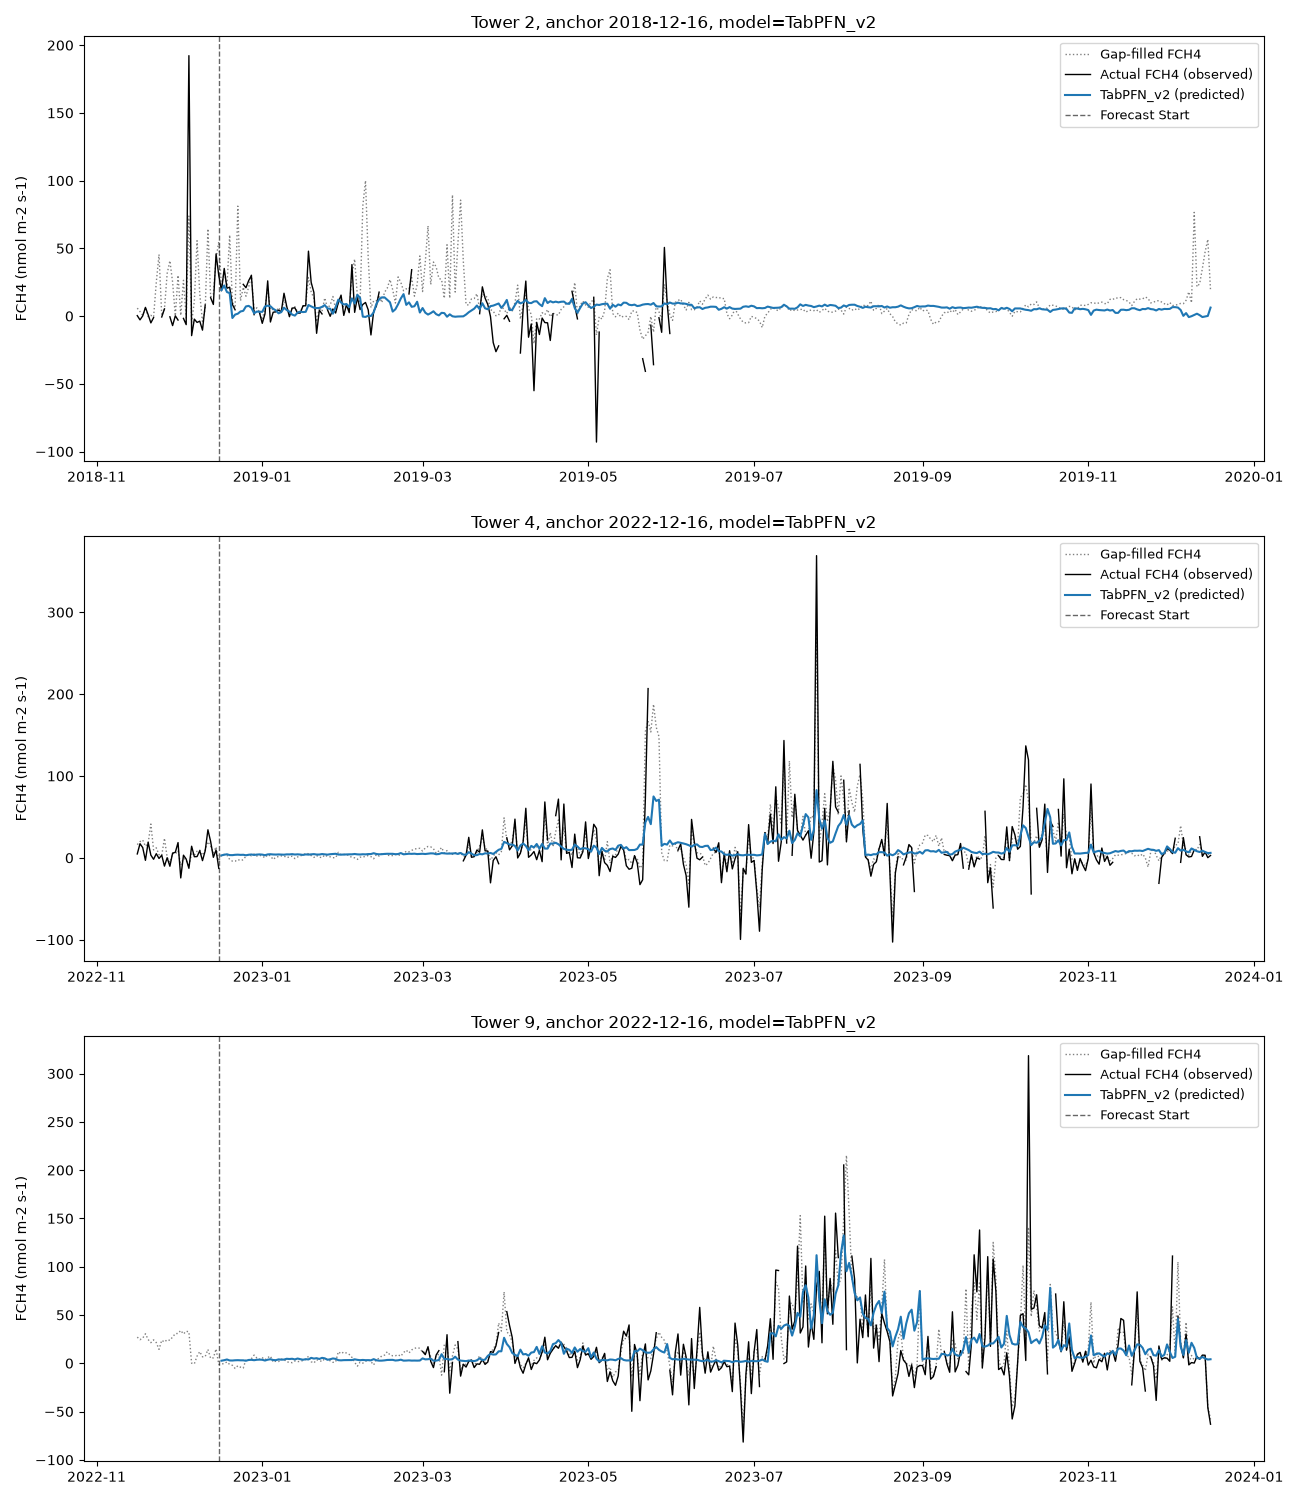
\includegraphics[width=0.92\textwidth]{Figures/ch5_champion_3towers.png}
\caption{Example 365-day recursive rollouts, all three towers, this dissertation's headline
configuration (equal-weight blend of three TabPFN variants). Tower 4 and Tower 9 (anchored December
2022) visibly track the rise and fall of several spike clusters, not just the low-flux baseline --
a clear qualitative improvement over this dissertation's earlier, un-refined TabPFN configuration.
Tower 2 (anchored December 2018, its only anchor with real observed data, Section 3.2.1) is included
for completeness.}
\end{figure}

\FloatBarrier

Tellingly, this same refinement pass confirms rather than resolves this chapter's central weakness:
scored on pre-anchor-estimated spike days specifically, the p95 event-corrected component's MASE
rises to 3.28, against 0.52 on non-spike days -- the spike-blindness problem quantified in full below
persists even after this targeted correction attempt.

DLinear and LSTM are decisively the weakest configurations tested, both performing far worse than
every tree, statistical, or foundation model in this comparison -- directly contradicting the
"simple linear models beat complex architectures" finding Zeng et al.\ report on standard benchmarks
(Section~\ref{sec:tabular-modelling}): on this dissertation's spike-dominated, non-stationary
target, model simplicity alone was not sufficient. TabICLv2's point-estimate result above reflects a
corrected extraction of its predicted median (the 0.5 quantile column) rather than its predicted
mean, which is materially biased high on this heavy-tailed, spike-dominated flux distribution; all
TabICLv2 numbers in this chapter use the corrected, median-based extraction.

A hyperparameter-tuning pass on LightGBM (rollout-specific tuning: reduced leaf count, minimum
child samples, and learning rate) found a real single-tower improvement that did not generalise: the
tuned configuration improved Tower 4's accuracy, but reusing the identical tuned hyperparameters at
Tower 9 produced a clear regression rather than a comparable gain -- a negative result
retained here specifically because it illustrates that hyperparameter tuning validated on one tower
cannot be assumed to transfer to another, reinforcing this dissertation's standing convention
(Chapter~\ref{Chap1}) of always reporting full three-tower coverage rather than a single-tower
result. Separately, in this dissertation's original, un-refined full-roster screen, TabPFN with
species-disaggregated features was effectively tied with a bodyweight-density variant (MASE=0.7150
vs.\ 0.7149) -- species-disaggregation is the configuration this dissertation's interpretability
work is built around (Section 5.3.4, Chapter~\ref{Chap6}), and remains so under the refined headline
configuration, whose \texttt{BASE+ALL} feature set includes species-disaggregated density as a
subset.

\subsection{Spike vs.\ Non-Spike Evaluation}

Table 5.1's aggregate MASE is pooled across every day of every rollout, and this masks a sharp,
practically important split in where that headline advantage actually comes from. This section
evaluates the standing headline configuration directly, then uses a finer-grained breakdown from
this dissertation's earlier, un-refined TabPFN configuration as a deep-dive supplement, since it
covers every tower individually and the headline configuration's own check confirms the identical
pattern at a coarser grain.

\paragraph{The standing headline configuration.} Using tower-specific 95th-percentile thresholds
estimated only from pre-anchor observations (a stricter cut than the 90th-percentile threshold used
in the deep-dive below), the p95 event-corrected component of this dissertation's headline blend
splits into 1,997 non-spike and 130 spike observed evaluation points, pooled across towers:

\begin{table}[htbp]
\centering
\begin{tabular}{lcc}
\toprule
Metric & Non-spike ($n=1{,}997$) & Spike ($n=130$) \\
\midrule
MASE & \textbf{0.524} & \textbf{3.285} \\
MAE & 20.31 & 176.48 \\
RMSE & 30.01 & 210.12 \\
Bias (prediction $-$ observation) & $+1.48$ & \textbf{$-176.48$} \\
\bottomrule
\end{tabular}
\caption{Spike-vs-non-spike performance, headline configuration's p95 event-corrected component
(observed target, pooled across towers).}
\end{table}

The pattern is unambiguous: MASE is a genuinely strong 0.524 on ordinary days but degrades to 3.285
on spike days -- over six times worse, and well above the seasonal-mean baseline (MASE$=1$) rather
than approaching it. This figure is not directly comparable in magnitude to the deep-dive's own
spike-day MASE below (which uses a looser 90th-percentile threshold covering a broader, less extreme
set of events) -- the qualitative conclusion, not the exact multiple, is what carries across both
thresholds: spike days remain this configuration's dominant failure mode. Bias is almost entirely a
spike-day phenomenon (average $-176.5$ nmol m\textsuperscript{-2} s\textsuperscript{-1} on spikes,
against a negligible $+1.5$ on non-spike days): the refinement pass that produced this dissertation's
headline result improved typical-day accuracy and partially corrected spike magnitude, but did not
close the underlying gap. The
remainder of this section uses the earlier configuration's per-tower saved daily chains to go
further than this pooled check allows -- percentile sensitivity, per-tower breakdown, and
spike-event detection -- while carrying the caveat above that its exact figures predate the
refinement.

\paragraph{Deep-dive (earlier, un-refined configuration).} This detailed breakdown
evaluates the champion configuration (TabPFN, BASE+species) separately on spike days -- defined
retrospectively as an observed daily FCH4 value at or above each tower's own 90th percentile, the
same definition used for the conditional-coverage check in Section~5.3.5 -- and on the remaining,
non-spike days. This is a diagnostic stratification on observed outcomes, not a deployable spike
detector, evaluated on the saved daily median forecast chains (\texttt{BASE+species}, all three
towers, anchors 2018--2022).

\begin{table}[htbp]
\centering
\begin{tabular}{lccc}
\toprule
Tower & 90th-percentile threshold & Non-spike $n$ & Spike $n$ \\
\midrule
T2 & 23.25 & 91 & 11 \\
T4 & 86.39 & 1{,}188 & 132 \\
T9 & 112.53 & 810 & 90 \\
\midrule
\textbf{Total} & tower-specific & \textbf{2{,}089} & \textbf{233} \\
\bottomrule
\end{tabular}
\caption{Spike/non-spike split by tower, 90th-percentile threshold.}
\end{table}

\begin{table}[htbp]
\centering
\footnotesize
\begin{tabular}{lcc}
\toprule
Metric & Non-spike & Spike \\
\midrule
Observed mean & 14.41 & \textbf{188.84} \\
Predicted mean & 14.84 & \textbf{32.69} \\
Bias (prediction $-$ observation) & $+0.43$ & \textbf{$-156.15$} \\
MAE & 19.38 & \textbf{156.15} \\
RMSE & 27.91 & \textbf{191.03} \\
Correlation & 0.329 & \textbf{0.131} \\
WAPE & 0.869 & 0.827 \\
Underprediction rate & 46.6\% & \textbf{100.0\%} \\
\bottomrule
\end{tabular}
\caption{Pooled point-forecast performance, non-spike vs.\ spike days.}
\end{table}

The mean spike prediction captures only 17.3\% of the mean observed spike magnitude, and every
single one of the 233 spike observations in this evaluation is underpredicted. WAPE looks
marginally better on spikes only because its denominator grows with observed magnitude -- absolute
error is in fact roughly eight times larger than on non-spike days.

\begin{table}[htbp]
\centering
\footnotesize
\begin{tabular}{lcc}
\toprule
Metric & Non-spike & Spike \\
\midrule
seasonal mean MASE & \textbf{0.659} & \textbf{1.001} \\
seasonal mean RMSSE & 0.699 & 0.995 \\
Persistence MASE & 0.911 & 0.909 \\
Native 90\% interval coverage & 84.3\% & \textbf{50.2\%} \\
Mean native interval width & 107.15 & 183.75 \\
Mean native pinball loss & 6.32 & \textbf{49.95} \\
\bottomrule
\end{tabular}
\caption{Baseline-scaled and uncertainty performance, non-spike vs.\ spike days.}
\end{table}

This table is the central finding of this deep-dive: this earlier configuration's own seasonal
mean-scaled MASE advantage (0.7150 pooled, no longer Table 5.1's top entry but still this
dissertation's most thoroughly spike-audited configuration) is concentrated almost entirely on
non-spike days (MASE 0.659, a genuine 34\% improvement over seasonal mean). On spike days the model
is effectively tied with the seasonal mean (MASE $\approx 1.001$) -- the model's advantage over a
naive seasonal baseline essentially disappears exactly on the days that matter most for the CH4
budget, the same qualitative conclusion the headline configuration's own coarser check reaches
above. Native
90\% interval coverage falls from 84.3\% to 50.2\% on spikes even though mean interval width
widens by about 72\%, and mean pinball loss rises almost eightfold; Conformalized Quantile
Regression, applied to this same champion configuration, improves spike coverage to approximately
57\% -- a real improvement over the raw figure above, but still well short of the nominal 90\%
target.

\begin{table}[htbp]
\centering
\footnotesize
\begin{tabular}{lcccc}
\toprule
Tower & MAE & Correlation & seasonal mean MASE & Native 90\% coverage \\
\midrule
T2 & 11.53 / 27.06 & 0.052 / 0.106 & 0.357 / \textbf{1.357} & 0.802 / 0.818 \\
T4 & 17.11 / 155.49 & 0.350 / 0.143 & 0.700 / \textbf{0.990} & 0.905 / 0.530 \\
T9 & 23.59 / 172.91 & 0.312 / \textbf{0.001} & 0.625 / \textbf{0.962} & 0.758 / 0.422 \\
\bottomrule
\end{tabular}
\caption{Tower-level non-spike / spike results. T2's 11 spike observations make its conditional
estimates unstable; T9's near-zero spike correlation indicates essentially no ability to track
spike-magnitude variation at that tower.}
\end{table}

A direct spike-\emph{detection} check -- flagging a predicted spike whenever the median forecast
itself exceeds the same tower-specific threshold used to label observed spikes -- confirms the
model is not merely imprecise on spike magnitude but structurally blind to spike \emph{occurrence}:
of 233 real spikes, only 1 is flagged as a true positive (recall 0.43\%, F1 = 0.008), against 2{,}086
true negatives (specificity 99.86\%). The model's apparent reliability comes entirely from correctly
predicting the much larger population of non-spike days, not from any genuine event-detection skill.
This conclusion is not an artefact of the 90th-percentile threshold choice: raising the definition
to the top 5\% (P95) sharpens it further -- observed spike magnitude rises from a mean of 128.64
(P80) to 257.33 (P95) while the mean prediction stays essentially flat at 30--35 throughout, and
native coverage degrades monotonically from 62.4\% to 35.9\%.

Taken together, this section supports a narrower reading of this dissertation's headline forecasting
result than the pooled MASE alone suggests, for both the deep-dive configuration and the current
standing headline alike. TabPFN-based models reduce typical-day absolute error relative to the
seasonal mean and are nearly unbiased across the bottom 90\% of the observed distribution, but do not
reliably reproduce, detect, or quantify methane spikes: on spike days their advantage relative to the
seasonal mean shrinks sharply or disappears, every spike in the deep-dive sample is underpredicted,
and calibrated uncertainty intervals undercover by roughly 40 percentage points. This is the central
limitation of this dissertation's forecasting contribution and is returned to explicitly in
Chapter~\ref{Chap7}.

\FloatBarrier

\subsection{Evaluation Against the Gap-Filled Target}

\begin{table}[h]
\centering
\footnotesize
\resizebox{\textwidth}{!}{%
\begin{tabular}{lcccc}
\toprule
Model & MASE (gap-filled) & RMSE & WAPE & Correlation \\
\midrule
Ensemble (MASE-weighted) & \textbf{0.666} & \textbf{25.38} & \textbf{0.704} & 0.522 \\
Ensemble (unweighted) & 0.666 & 25.39 & 0.705 & 0.523 \\
XGBoost & 0.677 & 25.87 & 0.725 & 0.477 \\
LightGBM & 0.689 & 26.11 & 0.728 & 0.496 \\
Random Forest & 0.703 & 25.85 & 0.756 & \textbf{0.529} \\
SARIMAX & 0.831 & 29.21 & 0.919 & 0.463 \\
TabPFN & 0.903 & 34.90 & 0.814 & 0.240 \\
TabICLv2 & 0.922 & 35.27 & 0.841 & 0.210 \\
TFT & 1.021 & 36.10 & 1.103 & 0.147 \\
LSTM & 1.122 & 39.79 & 1.188 & 0.185 \\
DLinear & 1.502 & 42.59 & 1.653 & 0.182 \\
\bottomrule
\end{tabular}%
}
\caption{The same model roster, scored against the gap-filled target instead of real observations
-- the ranking reverses, as flagged in Section 5.1.3.}
\end{table}

Scoring against the gap-filled target reverses Table 5.1's ranking almost exactly: the ensemble,
tree, and SARIMAX models now lead, and TabPFN/TabICLv2 fall to the middle of the pack. This is not
evidence that the gap-filled target is a more truthful evaluation -- it demonstrates that locally
fitted ensembles track the smoother, gap-filled reconstruction they are trained to regress onto more
closely, whereas the zero-shot foundation models see no equivalent benefit, exactly the circularity
risk flagged in Section 5.1.3. Table 5.1's observed-target ranking remains this dissertation's
authoritative comparison throughout.

\subsection{Interpretability}

Interpretability analysis converges on a single, repeatedly-confirmed finding across every method
capable of producing feature attributions on this model roster: livestock density is the dominant
driver of FCH4 at NWFP. This holds under native tree-model feature importance and SHAP attribution
(Random Forest, XGBoost, LightGBM), SARIMAX regression coefficients, and TabPFN permutation
importance, at every tower except Tower 2. SHAP importance for livestock density
grows with forecast lead time rather than shrinking, from a mean $|\text{SHAP}|$ of 7.6 at 1--7 days
to 38.4 at 181--270 days (Tower 4) -- livestock presence becomes a stronger, not weaker, predictor
the further into the future a forecast reaches.

The permutation-importance pass below targets this chapter's headline blend's own single-model
component specifically -- the p95 event-corrected direct-regression TabPFN champion
(\texttt{BASE\_ALL\_52}, MASE 0.6924, Section 5.3.1) -- rather than the earlier, now-superseded
TS-wrapper TabPFN+species configuration. \texttt{fx\_lsu\_dens} (combined livestock density) again
leads the overall ranking by a wide margin (mean importance 1.746), but species-disaggregation now
places a bodyweight-density feature absent from the earlier configuration's own feature
set -- \texttt{fx\_total\_liveweight\_dens} -- directly behind it (1.652), with \texttt{fx\_cattle\_dens}
close behind in third (1.550): cattle-driven livestock density remains a clear top-3 signal, though
no longer literally "the" second-ranked feature once this richer feature set's own bodyweight-density
term is included. Grazing activity, wind speed, and friction velocity round out the next several
ranks (\texttt{fx\_grazing\_active} 0.595, \texttt{fx\_WS\_mean} 0.498, \texttt{fx\_USTAR\_mean}
0.314). One genuine new wrinkle emerges under this architecture that was not present in the earlier
pass: \texttt{fx\_lamb\_dens} jumps to 8th overall (0.280), against near-bottom in the earlier
configuration, while \texttt{fx\_sheep\_dens} stays low (0.034) -- this dissertation flags it as a
plausible artefact of the pooled, tower-dummy-encoded architecture (which can pick up cross-tower
sensitivity patterns a per-tower time-series wrapper cannot) rather than a substantive new finding,
and it does not change the headline cattle-dominance conclusion.

Per-tower, Towers 4 and 9 both reproduce the identical top-3 ordering seen overall (Tower 4:
\texttt{fx\_lsu\_dens} 2.864, \texttt{fx\_total\_liveweight\_dens} 2.618, \texttt{fx\_cattle\_dens}
2.433; Tower 9: 2.372, 2.334, 2.216 respectively) -- overwhelming livestock dominance at both.
Tower 2's own top-10, by contrast, contains zero livestock features under this architecture either,
the same finding as every prior interpretability pass on this project, though its specific
composition is meteorological, hydrological, and management-recency rather than purely thermal: wind
speed and friction velocity lead (\texttt{fx\_WS\_mean}, \texttt{fx\_USTAR\_mean}), followed by
vapour-pressure deficit, catchment flow (7- and 14-day rolling means), fertiliser application rate
and recency, shortwave radiation, lagged soil moisture, and day-of-year phase -- consistent with
Tower 2's own muted livestock signal established in Section 4.5.3 and returned to in
Chapter~\ref{Chap6}, even though the exact meteorological drivers involved differ from the earlier
configuration's own top-10.

\begin{figure}[htbp]
\centering

\includegraphics[width=0.8\textwidth]{Figures/ch5_i03b_overall_ranking.png}
\caption{p95 event-corrected TabPFN champion (\texttt{BASE\_ALL\_52}): permutation feature
importance, pooled across all three towers and five rollout anchors. Livestock-related features
(red) dominate the top of the ranking.}
\end{figure}

\begin{figure}[htbp]
\centering

\includegraphics[width=\textwidth]{Figures/ch5_i03b_per_tower_top8.png}
\caption{Per-tower top-8 permutation importance. Tower 2's top features are exclusively
meteorological, hydrological, and management-recency (wind speed, friction velocity, vapour-pressure
deficit, catchment flow, fertiliser recency); Towers 4 and 9 both lead with livestock density and
cattle density specifically.}
\end{figure}

\begin{figure}[htbp]
\centering

\includegraphics[width=0.75\textwidth]{Figures/ch5_i03b_species_split.png}
\caption{Species-disaggregated livestock-density importance: cattle density drives most of the
species-split gain, though lamb density is a notable, unexplained exception (main text) and sheep
density stays low.}
\end{figure}

\FloatBarrier

One tower-level detail is worth reporting separately, with an explicit metric-convention warning:
evaluated per-tower with MASE scaled against chain-\emph{persistence} rather than seasonal mean (a
different, non-interchangeable convention from every MASE figure elsewhere in this chapter, per
Section 5.1.1), the earlier, un-refined TabPFN+species configuration achieves persistence-MASE of
0.229 at Tower 2, 0.883 at Tower 4, and 0.897 at Tower 9. Tower 2's very low error magnitude here
should not be read as a genuinely easier forecasting task: it reflects a much smaller and
structurally different target distribution together with a small evaluation sample (102 rows), not
better model tracking -- consistent with Tower 2's established livestock-blindness (this section,
above) rather than any underlying ease.

\subsection{Uncertainty Quantification}

Uncertainty quantification in this chapter proceeds in two stages: a first, broad comparison across
eight model families to establish general calibration behaviour, followed by a champion-focused
recalibration on TabPFN and TabICLv2 specifically, and finally two targeted diagnostics -- spike
coverage and livestock-density-stratified calibration -- on the champion pair. As throughout this
dissertation, Area-of-Applicability is not used as an uncertainty-quantification method; PICP
(Prediction Interval Coverage Probability) and MPIW (Mean Prediction Interval Width) are the primary
uncertainty vocabulary, alongside pinball loss for the quantile-based comparisons below. Raw model
quantiles are passed through leave-one-anchor-out conformal calibration -- each of the five rollout
anchors takes a turn as the calibration set for the other four -- targeting 90\% nominal coverage.

\subsubsection{All-Model Uncertainty Comparison}

\begin{table}[h]
\centering
\footnotesize
\resizebox{\textwidth}{!}{%
\begin{tabular}{lccccccc}
\toprule
Model & $n$ & Raw PICP & Raw MPIW & Raw pinball & Conf.\ PICP & Conf.\ MPIW & Conf.\ pinball \\
\midrule
Ensemble (unweighted) & 2217 & 0.732 & 78.82 & 10.47 & 0.890 & \textbf{145.28} & \textbf{10.53} \\
Ensemble (MASE-weighted) & 2217 & 0.728 & 77.98 & 10.48 & 0.892 & 145.31 & \textbf{10.53} \\
Random Forest & 2217 & 0.379 & 47.18 & 12.23 & 0.886 & 145.77 & \textbf{10.53} \\
LightGBM & 2217 & 0.489 & 55.22 & 11.38 & \textbf{0.894} & 149.79 & 10.70 \\
XGBoost & 2217 & 0.485 & 56.36 & 11.38 & 0.891 & 148.67 & 10.74 \\
SARIMAX & 2217 & 0.871 & 156.52 & 11.17 & 0.892 & 158.65 & 11.04 \\
TFT & 2217 & 0.839 & 145.63 & 10.92 & \textbf{0.894} & 162.89 & 11.49 \\
TabPFN & 2217 & 0.807 & 120.31 & 11.18 & 0.892 & 165.42 & 11.55 \\
\bottomrule
\end{tabular}%
}
\caption{First-stage uncertainty comparison, T4/T9 pooled test rows (Tower 2 lacked sufficient
calibration support). Raw quantiles as produced by each model, and the same after leave-one-anchor-
out conformal calibration.}
\end{table}

Raw calibration quality varies sharply by model family before any correction is applied: tree models
(Random Forest, LightGBM, XGBoost) are badly overconfident (raw PICP 0.38--0.49, far below the 0.90
target), while SARIMAX, TFT, and TabPFN start much closer to nominal (raw PICP 0.81--0.87). Conformal
calibration equalises marginal coverage across every model family (0.886--0.894 after calibration),
but achieves this primarily by widening the previously overconfident tree models' intervals, not by
narrowing anything materially. The ensembles and Random Forest achieve the lowest conformal pinball
loss (10.53) in this first, broad comparison, marginally ahead of the champion-focused models
examined next.

\subsubsection{Conformal Calibration for Best Models}

\begin{table}[h]
\centering
\footnotesize
\begin{tabular}{llccccc}
\toprule
Model & Tower & $n$ & Raw PICP & Conf.\ PICP & Conf.\ MPIW & Conf.\ pinball \\
\midrule
\textbf{TabPFN (B18 champion)} & T4 & 1318 & 0.929 & 0.898 & \textbf{144.5} & \textbf{10.09} \\
\textbf{TabPFN (B18 champion)} & T9 & 899 & 0.928 & 0.894 & 166.4 & 11.42 \\
TabICLv2 (Ch5 champion) & T4 & 1318 & 0.964 & 0.895 & 154.7 & 10.63 \\
TabICLv2 (Ch5 champion) & T9 & 899 & 0.771 & 0.894 & 195.3 & 13.04 \\
TabICLv2 (scenario-safe)\textsuperscript{\ddag} & T4 & 1318 & 0.959 & 0.895 & 151.3 & 10.71 \\
TabICLv2 (scenario-safe)\textsuperscript{\ddag} & T9 & 704 & 0.991 & 0.884 & 161.2 & 11.47 \\
\bottomrule
\end{tabular}
\caption{Champion-focused conformal recalibration. \textsuperscript{\ddag}\texttt{Direct\_TabICLv2\_solo\_trend}
on the restricted \texttt{FX\_A\_SPECIES} feature set -- the actual scenario-projection engine used
in Chapter~\ref{Chap6}, distinct from this chapter's own TabICLv2 champion configuration.}
\end{table}

Recalibrating specifically on the champion configurations narrows the comparison to the models this
dissertation actually recommends for forecasting (TabPFN, TabICLv2) and for scenario projection
(the restricted-feature TabICLv2 variant above). Tower 2 cannot support calibration at all in any of
these three passes -- too few real observed values fall inside its rollout anchor windows to build a
usable calibration set, the same structural limitation identified for Tower 2 throughout this
dissertation (raw-only figures: TabPFN B18 champion PICP 0.726/MPIW 86.0, $n=102$; scenario-safe
TabICLv2 PICP 0.804/MPIW 182.9, $n=102$). Recalibrated specifically for B18's actual champion
architecture (direct \texttt{BASE\_ALL\_52} regression plus the p95 spike-gate, rather than the
earlier TS-wrapper configuration), TabPFN's raw PICP now starts much closer to nominal at both towers
(0.929/0.928, against 0.867/0.724 under the earlier configuration) -- plausibly because the richer,
52-column feature set's native quantile spread is better calibrated before any correction is applied.
After conformal calibration, all three model/tower combinations converge close to the 0.90 target
(0.884--0.898), as intended, and B18's TabPFN champion is now the sharpest and best-scored of the
three once calibrated (MPIW 144.5/166.4, pinball 10.09/11.42) -- a modest but genuine improvement
over both its own earlier-configuration numbers and TabICLv2's. The scenario-safe TabICLv2 variant,
despite its deliberately restricted 13-feature set, calibrates to essentially the same standard as
the two full-feature champions (conf.\ PICP 0.895/0.884, MPIW 151.3/161.2) -- reassuring given that
this is the specific configuration Chapter~\ref{Chap6}'s scenario projections actually depend on.

\begin{figure}[htbp]
\centering
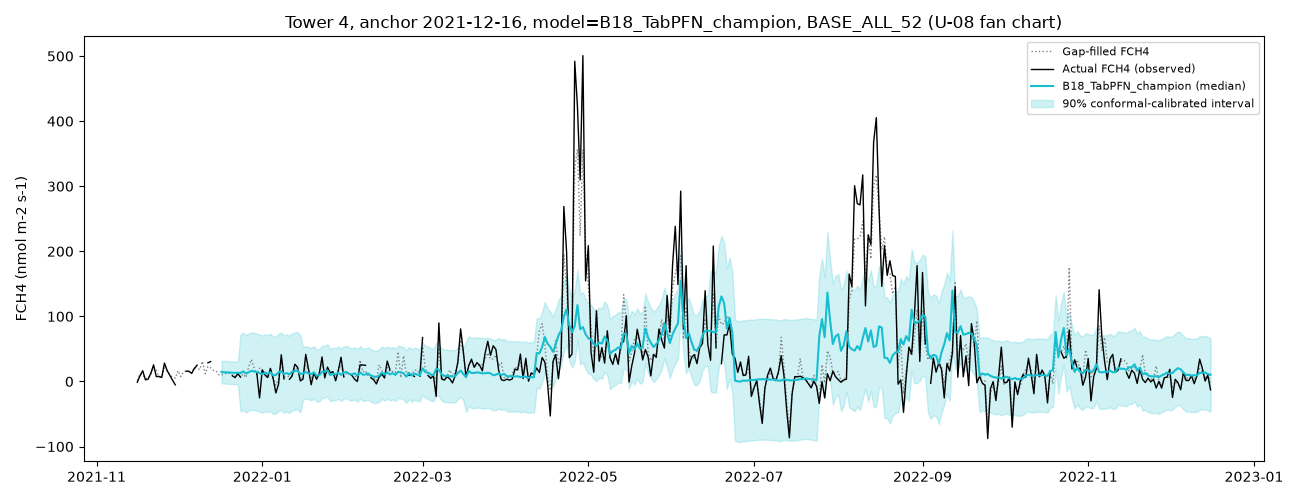
\includegraphics[width=\textwidth]{Figures/ch5_u08_fanchart_T4.png}
\caption{Fan chart, Tower 4, anchor December 2021, B18's TabPFN champion (\texttt{BASE\_ALL\_52}):
median forecast and 90\% conformal-calibrated interval against observed and gap-filled FCH4. The
interval widens visibly during the mid-year, high-livestock-density window and still does not
fully contain every large spike -- the motivation for the CQR spike-coverage correction below.}
\end{figure}

\FloatBarrier

\subsubsection{Spike-Coverage Correction (CQR)}

The fan chart above motivates a direct question this dissertation can now answer quantitatively:
does Conformalized Quantile Regression (CQR), applied specifically to widen intervals conditional on
predicted spike risk, meaningfully close the spike-undercoverage gap identified throughout this
chapter (Section~5.3.2)? Applying CQR to both champion-tier models' saved chains gives a clear yes:

\begin{table}[h]
\centering
\footnotesize
\resizebox{\textwidth}{!}{%
\begin{tabular}{lcccc}
\toprule
Model & Spike coverage (raw) & Spike coverage (CQR) & Non-spike coverage (raw) & Non-spike coverage (CQR) \\
\midrule
TabPFN (B18 champion) & 0.266 & \textbf{0.775} & 0.966 & 0.879 \\
TabICLv2 (scenario-safe) & 0.266 & \textbf{0.901} & 0.961 & 0.832 \\
\bottomrule
\end{tabular}%
}
\caption{Spike-day interval coverage before and after CQR correction, both champion-tier models.}
\end{table}

Both models' raw, uncalibrated spike coverage sits at a near-identical 26.6\% -- markedly worse than
the deep-dive TabPFN+species configuration's own raw spike coverage reported in Section~5.3.2
(50.2\%), a reminder that raw interval width alone is not a stable quantity across configurations.
CQR correction roughly triples spike coverage for both models (to 77.5\% for the B18 champion and
90.1\% for the scenario-safe TabICLv2 variant), at a real but modest cost to non-spike coverage
(0.966$\to$0.879 and 0.961$\to$0.832 respectively) -- intervals widen selectively where spike risk is
predicted to be high, trading a small amount of everyday-day coverage for a large gain exactly where
this chapter's central limitation (Section~5.3.2, Chapter~\ref{Chap7}) is sharpest. This meaningfully
updates the picture from the deep-dive configuration's own CQR result (spike coverage improved only
to approximately 57\%, Section~5.3.2): applied to either current champion-tier model, CQR now closes
most, not merely some, of the nominal-coverage gap on the days that matter most for the CH4 budget.

\begin{figure}[htbp]
\centering
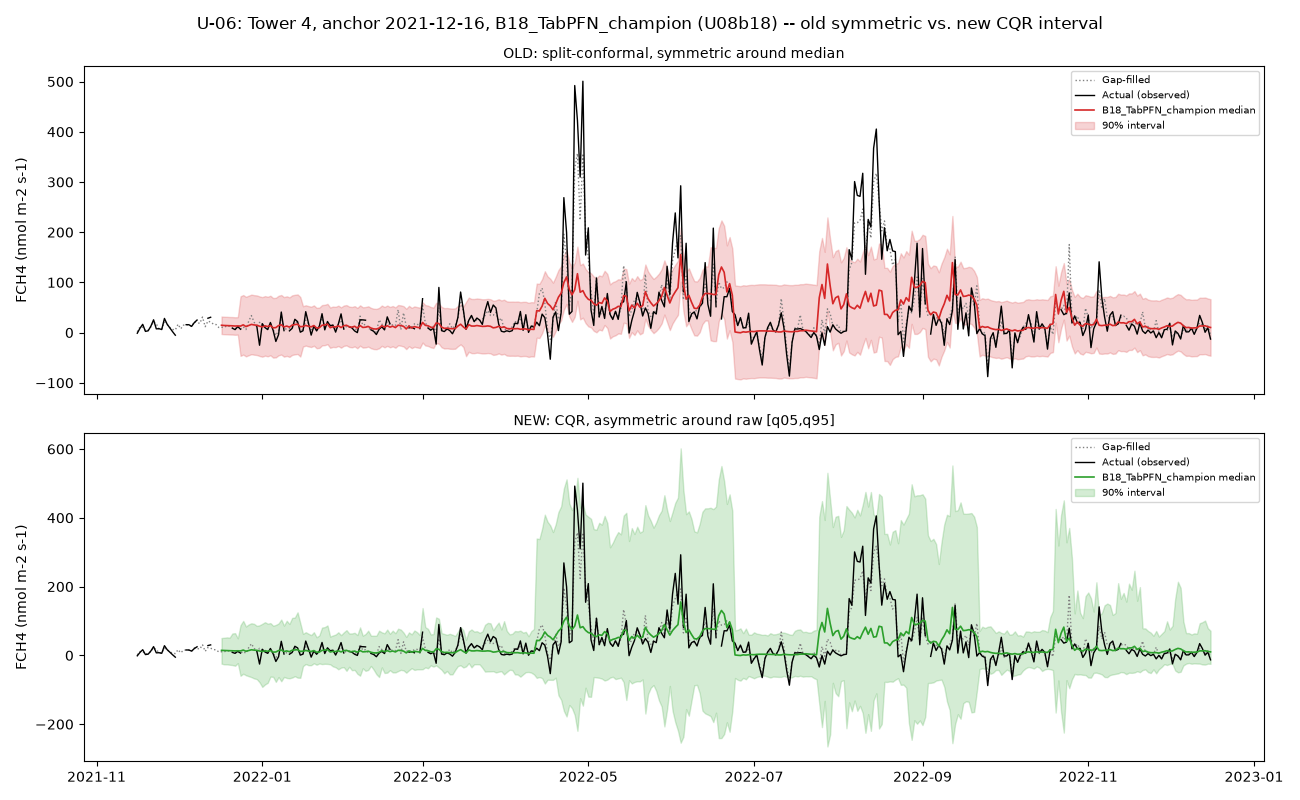
\includegraphics[width=\textwidth]{Figures/ch5_cqr_spike_T4.png}
\caption{Tower 4, anchor December 2021, B18's TabPFN champion: raw vs.\ CQR-corrected prediction
intervals around observed and gap-filled FCH4, illustrating the selective widening that produces
the spike-coverage gain in the table above.}
\end{figure}

The table above pools Towers 4 and 9 only, consistent with every conformal-calibration result in
this chapter (Section 5.3.5.2) -- Tower 2 cannot support the leave-one-anchor-out calibration step at
all. This is stated in prose throughout this chapter but has not, until now, been shown directly:

\begin{figure}[htbp]
\centering
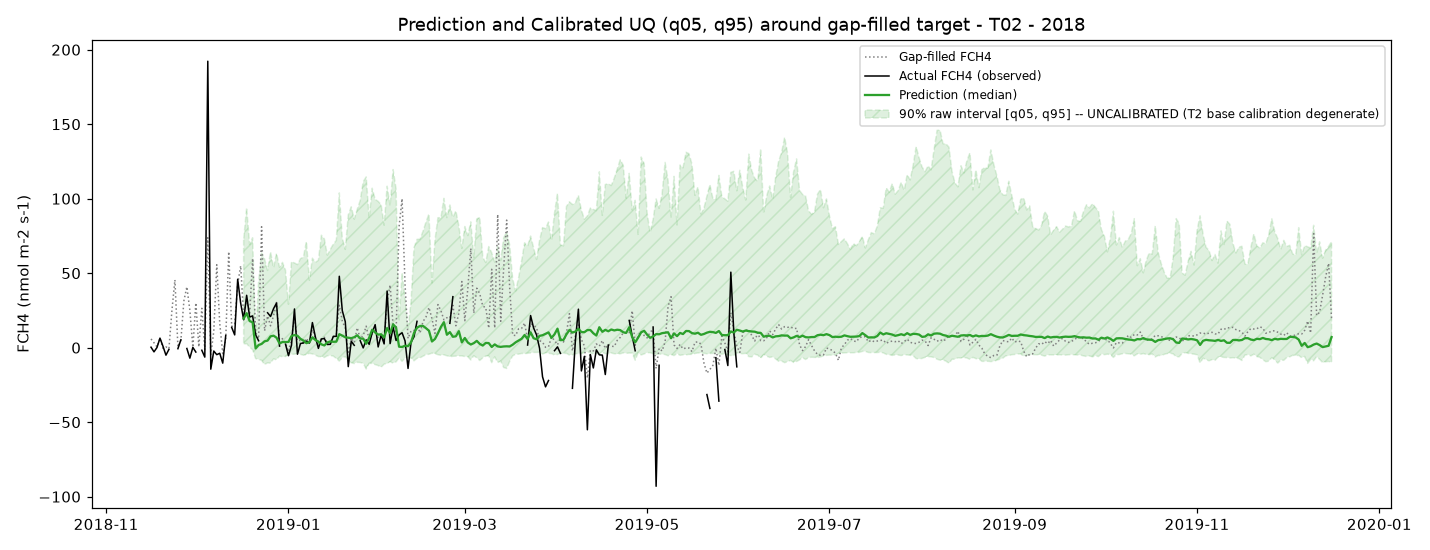
\includegraphics[width=\textwidth]{Figures/ch5_cqr_spike_T2.png}
\caption{Tower 2, anchor December 2018 (its only anchor with real observed data,
Section~3.2.1): the model's raw, \emph{uncalibrated} $[q_{05}, q_{95}]$ interval, shown hatched to
distinguish it from the CQR-calibrated bands at Towers 4 and 9 above. No CQR margin exists for
Tower 2 at any anchor -- this is what "Tower 2 cannot support calibration" actually looks like,
not a narrower version of the calibrated case.}
\end{figure}

Both figures above are drawn from a full three-tower, five-anchor set (15 total figures, one per
tower-anchor combination) generated for this dissertation's own verification, consistent with this
project's standing full-coverage convention (Chapter~\ref{Chap1}); the two shown here are the
representative examples, and the pooled Tower 4/9 table above already reflects all fifteen
combinations, not just the anchor illustrated.

\FloatBarrier

\subsubsection{Livestock-Conditional Uncertainty}

Section~5.3.2's spike-vs-non-spike split conditions on the observed \emph{outcome}. A
complementary, forward-looking stratification instead conditions on livestock density itself --
an input known before the fact, motivated directly by this chapter's own interpretability finding
(Section 5.3.4) that livestock density is the dominant driver of FCH4:

\begin{table}[h]
\centering
\footnotesize
\begin{tabular}{llcccc}
\toprule
Model & LSU tier & $n$ & PICP & MPIW & Pinball \\
\midrule
TabPFN (B18 champion) & Low & 855 & 0.885 & 91.4 & 4.73 \\
TabPFN (B18 champion) & Mid & 466 & 0.882 & 108.7 & 5.39 \\
TabPFN (B18 champion) & High & 875 & 0.825 & 305.2 & 17.32 \\
TabICLv2 (scenario-safe) & Low & 811 & 0.836 & 166.8 & 6.53 \\
TabICLv2 (scenario-safe) & Mid & 383 & 0.833 & 213.3 & 6.84 \\
TabICLv2 (scenario-safe) & High & 807 & 0.865 & 381.8 & 17.37 \\
\bottomrule
\end{tabular}
\caption{Livestock-density-stratified CQR coverage, width, and pinball loss, both champion-tier
models.}
\end{table}

Interval width and pinball loss both grow sharply with livestock-density tier for both models --
roughly 3.3$\times$ wider at the high tier than the low tier for the B18 champion and 2.3$\times$ for
the scenario-safe TabICLv2 variant -- directly quantifying the regime-dependent uncertainty this
chapter's interpretability work already identifies as the dominant source of predictive difficulty.
Coverage stays close to, and for the B18 champion's low/mid tiers slightly above, the earlier
deep-dive configuration's own figures, remaining modestly below the nominal 0.90 target in every tier
for both models (0.825--0.885) -- a residual gap this dissertation reports honestly rather than
tuning away, since narrowing it further would risk re-introducing the spike-undercoverage problem
quantified in Section~5.3.2 and directly above.

\begin{figure}[htbp]
\centering
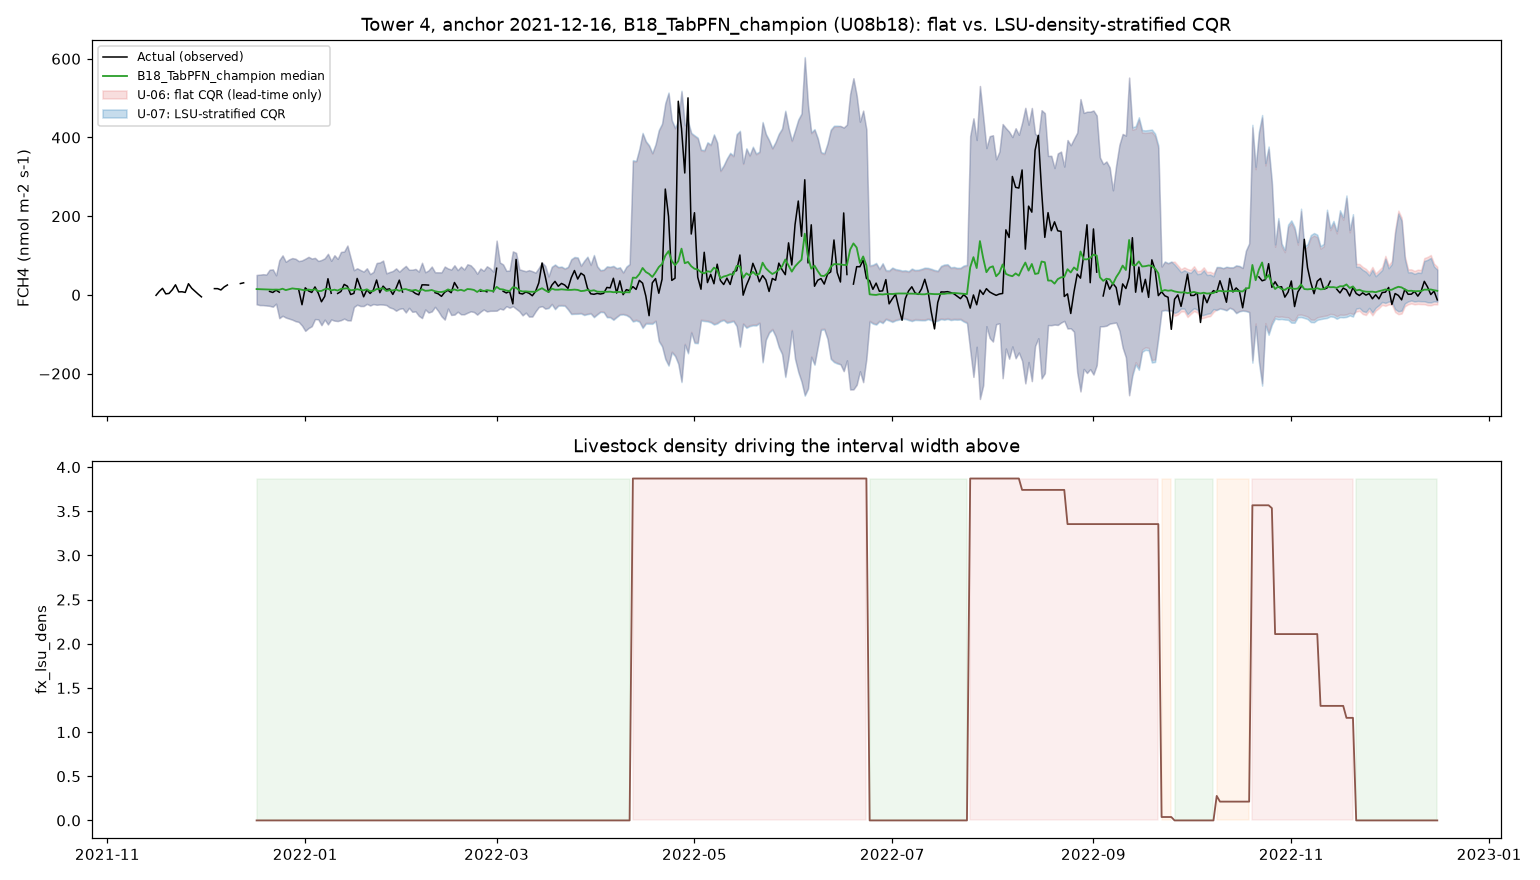
\includegraphics[width=\textwidth]{Figures/ch5_lsu_cqr_T4.png}
\caption{Tower 4, anchor December 2021: flat CQR (lead-time-only margin) vs.\
livestock-density-stratified CQR intervals, with the underlying \texttt{fx\_lsu\_dens} trajectory
shown below -- the stratified interval visibly widens exactly where livestock density is high,
independent of which specific model produced the underlying point forecast.}
\end{figure}

\FloatBarrier

\FloatBarrier
